%Präambel
\documentclass[paper=a4,fontsize=11pt,headsepline,footsepline,parskip=half]{scrartcl}
\usepackage[utf8]{inputenc}
\usepackage[T1]{fontenc}
\usepackage{amsmath,amsfonts,amssymb}
\usepackage{ngerman,graphicx,textcomp,mathpazo,booktabs}
\usepackage[decimalsymbol=comma,per=frac]{siunitx}
\usepackage[textfont=sl,labelfont=bf]{caption}

%Seite einrichten
\areaset[2cm]		% Zusätzlicher Rand für die Bindung
        {17cm}{24cm}	% Textbreite und -Höhe

%Zeilenabstand
\linespread{1.2} %Standardwert

%Kopf- und Fußzeile
\usepackage{scrlayer-scrpage}
\setlength{\headheight}{23pt}
\lohead{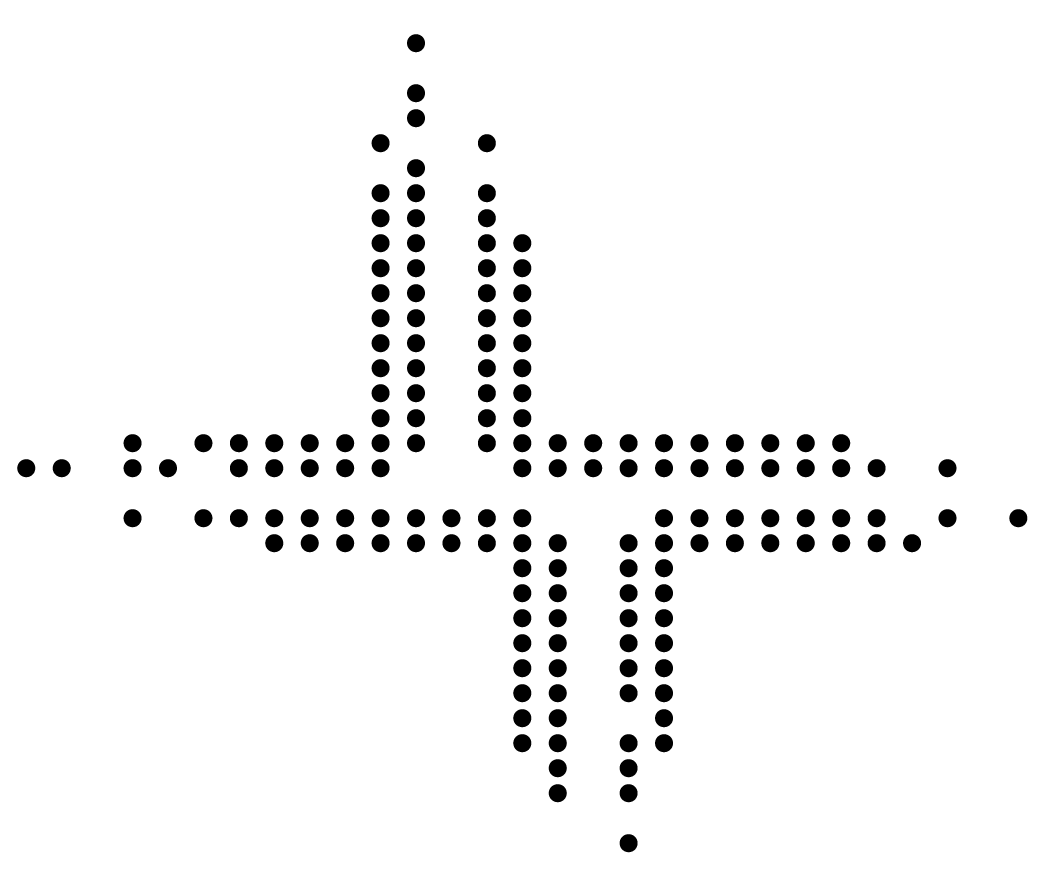
\includegraphics[width=0.7cm]{../logofbi} Hochschule Darmstadt}
\rohead{David Falk, Christian Lichtsinn}
\pagestyle{scrheadings}

%sollte als letztes Paket geladen werden
\usepackage{hyperref}

\begin{document}

%Titelblatt
\begin{titlepage}

\begin{minipage}[c]{5cm}
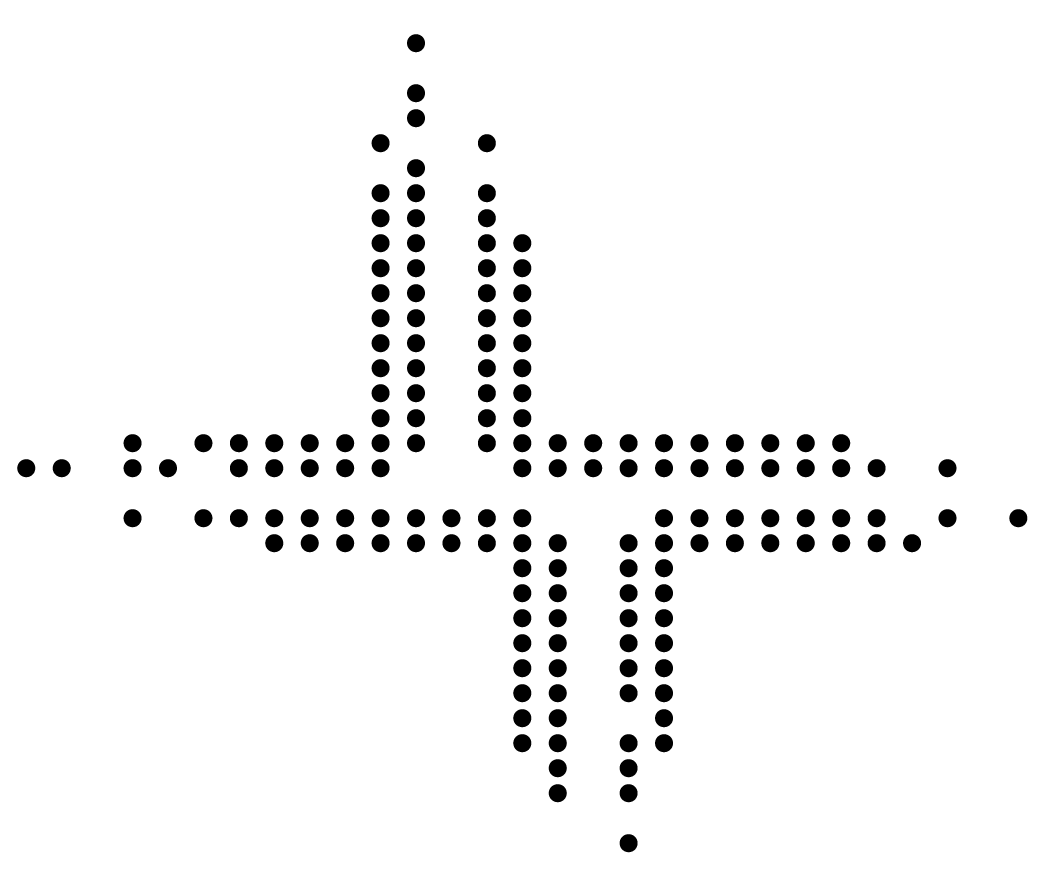
\includegraphics[width=5cm]{../logofbi}
\end{minipage}
\hfill
\begin{minipage}[c]{10cm}
\begin{flushright}
\Large Einführung in die Technik\\und Anwendung von\\
\LARGE \textbf{RFID}
\end{flushright}
\end{minipage}

\vspace*{1cm}

\begin{minipage}[c]{9cm}
\begin{flushleft}
\large David Falk (736532)\\Christian Lichtsinn (736787)\\Praktikum 3: 16.11.15: \textbf{Mo-56x}
\end{flushleft}
\end{minipage}
\hfill
\begin{minipage}[c]{7cm}
\begin{flushright}
\large Betreuer:\\Prof. Ralf S. Mayer\\F. Dotzauer
\end{flushright}
\end{minipage}

\vspace*{1cm}

%Workaround nötig wegen parskip Option.
\begingroup
  \setlength{\parskip}{0pt}% keinen Absatzabstand einfügen
  \setlength{\parindent}{0pt}% nicht einziehen
  \setlength{\parfillskip}{0pt plus 1fil}% Absatz darf komplett gefüllt sein
  \par\rule{\linewidth}{1.5pt}\par
\endgroup

\vspace*{1cm}

\noindent
\large{Thema: \textbf{RFID LF Reader und Transponder}}

%KAPITEL 1
\section{Fragen zu Atmel ATA2270-EK1}

\subsection{Wann darf das Reader-Board erst eingeschaltet werden?}

Erst wenn Reader-Board, die $125 kHz$-Antenne, sowie die Stromversorgung korrekt am Mainboard angebracht wurden, darf man das Reader-Board einschalten.

\subsection{Welche Spannung an der Spule ist zu erwarten?}

Es ist eine Spannung von $200 V$ zu erwarten.

\subsection{Wie ist die Induktivität der Antennenspule? Wie groß etwa wäre die dazugehörige Kapazität auf der Leser-Platine?}

Die Induktivität der Antennenspule wird mit $700 \mu H$ angegeben. Bei einer Resonanzfrequenz von $\omega_r = 125 kHz$ ergibt sich mit

\end{titlepage}

\begin{align}
 \omega_r = \frac{1}{\sqrt{LC}} \Leftrightarrow C = \frac{1}{L \cdot \omega_r^2}
\end{align}

für die Kapazität $C = 91,429 nF$ auf der Leser-Platine.

\subsection{Was wäre zu beobachten, wenn eine andere Antennenspule mit unterschiedliicher Induktivität angeschlossen würde?}

Man müsste einen anderen Kondensator wählen, damit die Resonanzfrequenz $\omega_r = 125 kHz$ erreicht wird.

\subsection{Ist die mitgelieferte Antenne optimal?}

Die Frage ist hier u.a. optimal wofür? Man kann die Antenne entweder für Reichweite oder (Bereich... TODO!) optimieren. Die mitgelieferte Antenne
ist ein Kompromiss aus beidem, daher kann man sagen, dass sie nicht optimiert ist.

\subsection{Woraus besteht ein Tag (Transponder) im vorliegenden Kit?}

Ein Tag besteht aus einem integrierten Schaltkreis (intregrated circuit, IC), einem Kondensator und einer Antennenspule.

\subsection{Wie ist die Reihenfolge der gespeicherten und übertragenen Bits? Welcher Endian? Little oder Big?}

Die Blockreihenfolge ist von links nach rechts von 1 bis 32. Big Endian?

\subsection{Muss ein Tag initialisiert werden? Wann?}

TODO

\subsection{Welche Eigenschaften hat ein TK5551-Transponder?}

Ein TK5551-Transponder hat einen Konfigurationsblock und 7 Datenblöcke, jeder Datenblock speichert 32 bits und damit insgesamt 224 bits.

\subsection{Welche Eigenschaften hat ein ATA5577-Transponder?}

Ein ATA5577-Transponder hat einen Konfigurationsblock, 7 Datenblöcke à 32 bits (zusammen 224 bits) und 2 ID-Blöcken, sowie einem konfigurierbaren
Analog-Frontend.

\subsection{Welche Besonderheiten hat ein ATA5570-Transponder?}

Je nachdem, ob die Impedanz hoch oder niedrig ist, werden die Daten korrekt oder invers versendet.

%KAPITEL 2
\section{Fragen zu SamSys-UHF-Reader}

\subsection{Wie ist das Lesegerät MP9320 in Betrieb zu nehmen, was ist zu beachten, wie wird die Antenne angeschlossen?}

Das Lesegerät verbindet man mit einem seriellem Kabel mit einem PC, damit man via einer Software mit dem Lesegerät kommunizieren kann. Das MP9320
darf dabei aber erst in Betrieb genommen werden, wenn entweder an den Antennenanschlüssen entsprechende UHF-RFID-Antennen angeschlossen sind oder
sich ein $50\ohm$-Abschlusswiderstand anstatt der Antenne befindet.

\subsection{Könnten mehrere UHF-Lesegeräte sich gegenseitig beeinflussen?}

Ja.

\subsection{Was bedeutet ISO 18000-6?}

ISO 18000-6 ist eine Norm für die Spezifikation der Luftschnittstelle im UHF-Bereich (Ultra High Frequency) von $860 MHz$ bis $960 MHz$. 

\subsection{Wie können Tags mit der RF Command Suite und der RS232-Schnittstelle gelesen werden?}

TODO

%KAPITEL 3


\end{document}
